\appendix


\section{Appendiks - Grunnleggende databladkunnskaper}\label{app:datablad}

For enhver mikrokontroller er det viktig å kunne mestre bruken av datablade. Mer spesifikt, er det veldig viktig for å forstå hvordan man bruker det som kalles memory mapped IO. I praksis, betyr memory mapped IO at man \verb|typecaster| adressen til en modul inn i en \verb|struct|. Grunnen til at man bruker memory mapped IO, er at det gjør det mulig å skrive direkte til registrene i mikrokontrolleren ved å bare endre på \verb|struct|-ens medlemsvariabler. Se forøvrig pensumlitteratur og forelesninger for mer informasjon om memory mapped IO og hvordan en forholder seg til det i \verb|C|-programmering.

\subsection{Memory Mapped IO informasjon fra datablad}
Det første man trenger for å kunne typecaste adressen til en modul inn i en \verb|struct|, er å finne adressen til modulen. I \verb|GPIO|-tilfellet, er baseadressen \verb|0x50000000| (se figur \ref{fig:app-gpio-modul}).


\begin{figure}[ht]
    \centering
    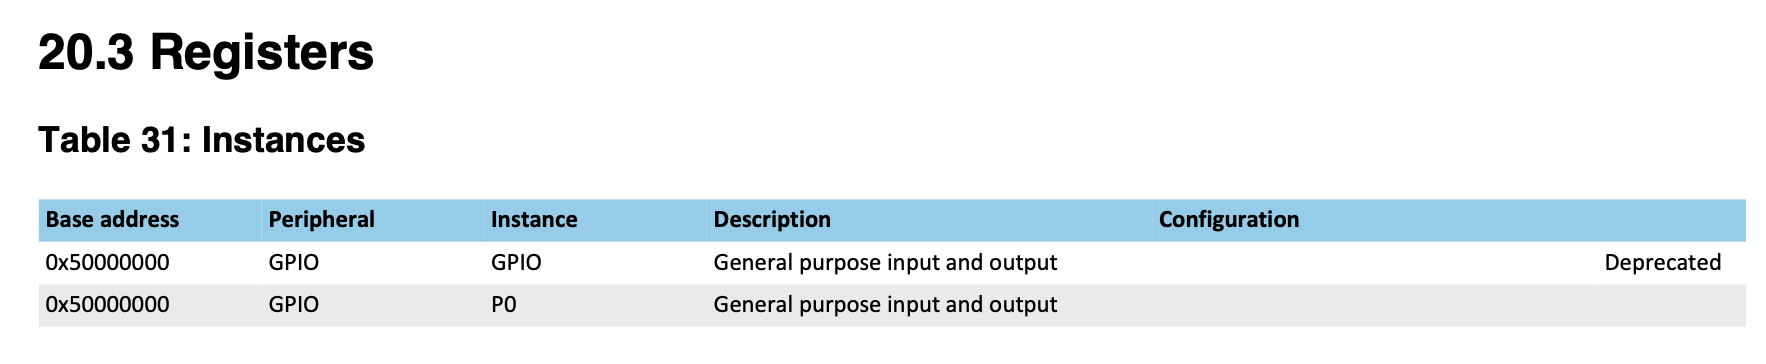
\includegraphics[scale=0.5]{Main/figures/gpio_addresse.png}
    \caption{Startsadressene til GPIO-modulene (side 116 fra \texttt{nrf52832 Product Specification.pdf}).}
    \label{fig:app-gpio-modul}
\end{figure}

Noen moduler kan ha flere \textit{instanser}. Et annet eksempel på dette er \verb|Timer|-modulen til nRF52-en. Der finnes det fem forskjellige kopier av samme enhet (se figur \ref{fig:app-timerl}). Dette er veldig nyttig dersom man ønsker for eksempel flere uavhengige klokker.

\begin{figure}[ht]
    \centering
    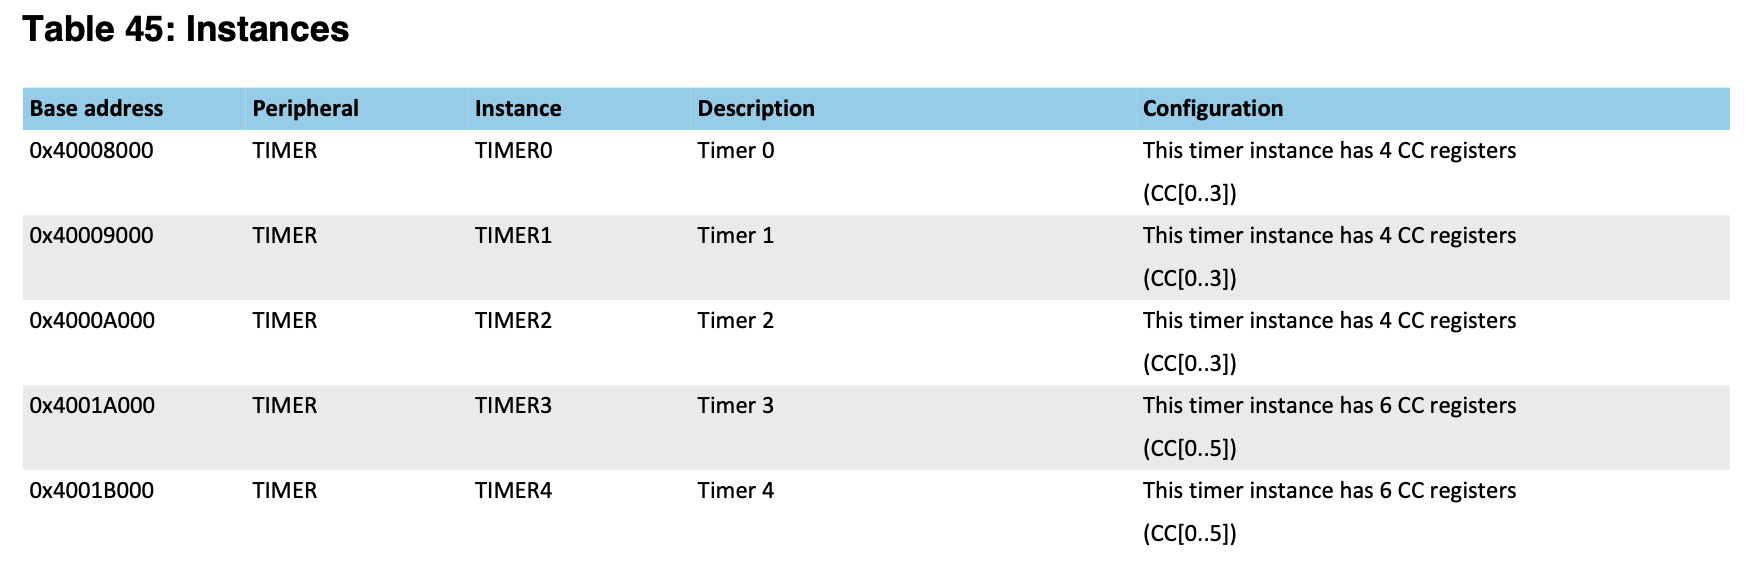
\includegraphics[scale=0.5]{figures/timer_memory.png}
    \caption{Startadressene til \texttt{Timer}-modulen (side 239 fra \texttt{nrf52832 Product Specification}).}
    \label{fig:app-timerl}
\end{figure}

Når man først har baseadressen, oversettes dette ganske direkte inn i \verb|C| slik:

\verb|#define GPIO0 ((NRF_GPIO_REG0*)0x50000000)|

Denne kodesnutten tilsvarer å definere instansen av \verb|GPIO| som en peker til adresse \verb|0x5000000|, hvor pekeren er av typen \verb|NRF_GPIO_REG0|. 

Neste steg er å definere hvordan \verb|NRF_GPIO_REG0| ser ut. Strukturen til \verb|NRF_ GPIO_REG0| finner man som oftest rett under baseadressen (se figur \ref{fig:app-memory-struct}).

\begin{figure}[ht]
    \centering
    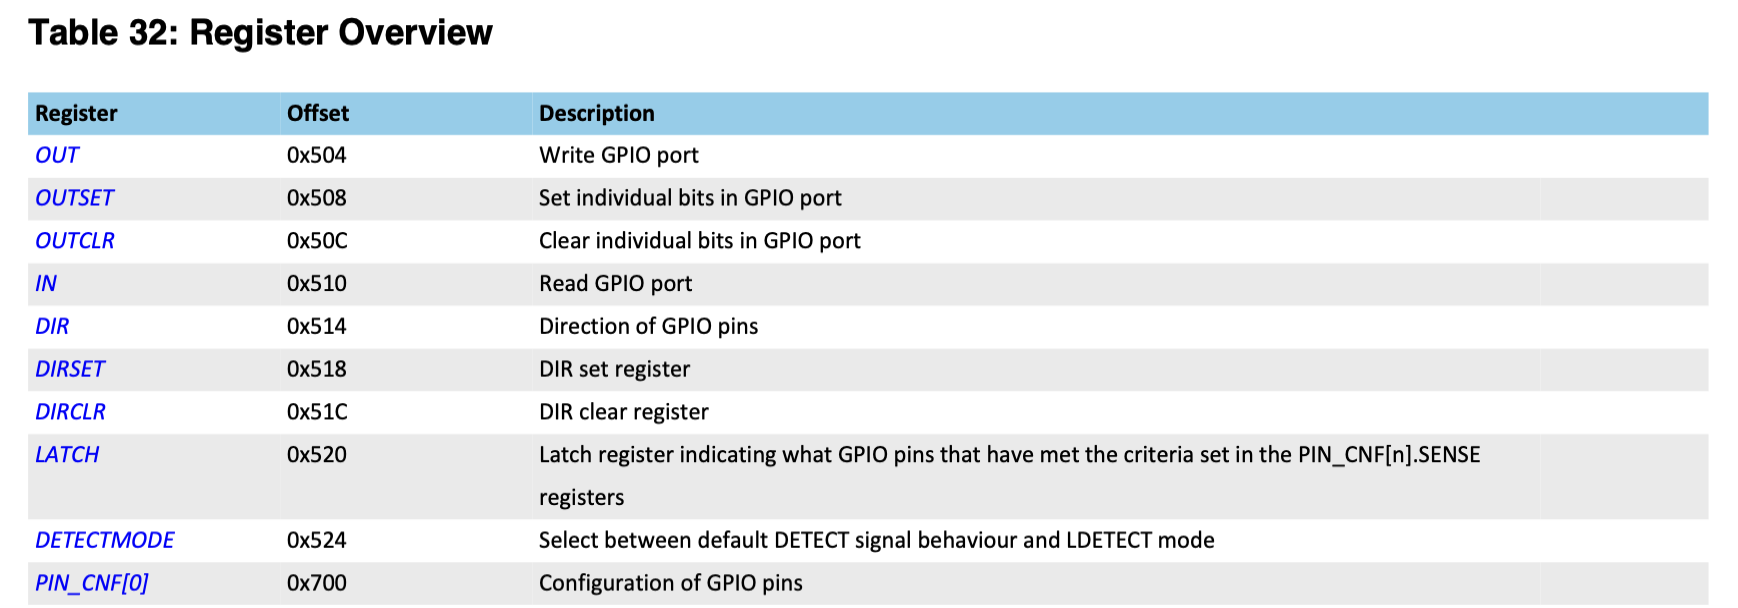
\includegraphics[scale=0.50]{figures/memory_stuff_gpio.png}
    \caption{Registrene i GPIO-modulene (side 117 fra \texttt{nrf52832 Product Specification}).}
    \label{fig:app-memory-struct}
\end{figure}

Informasjonen som vi trenger for å kunne bruke \verb|NRF_GPIO_REG0| sine registre finner man under \verb|Register| og \verb|Offset|. \verb|Register| beskriver navnet til registrene som finnes i modulen, mens \verb|Offset| beskriver offsetet mellom et register, og det registeret som kom før. Eksempelvis vil man for \verb|GPIO|-modulen kunne se at registeret \verb|OUT| har et offset på \verb|0x504|. Dette betyr at registeret ligger $504_{16} = 1284_{10}$ byte unna forrige register. Siden det ikke ligger noe register før \verb|OUT| i \verb|GPIO|-modulen, betyr dette at det er $1284_{10}$ byte mellom baseadressen til modulen og \verb|OUT|. I \verb|C| kan man definere \verb|NRF_GPIO_REG0|-\verb|struct|-en slik:

\begin{lstlisting}
typedef struct{
volatile uint32_t RESERVED0[321];
volatile uint32_t OUT;
...
} NRF_GPIO_REG0;
\end{lstlisting}

Grunnen til at vi skriver 321 og ikke 1284 er at hvert element i et array av typen \verb|uint32_t| er 32 bit stort - altså 4 bytes - noe som tilsvarer registerstørrelsen i prosessoren. Registerstørrelsen i en prosessor er platform-spesifikk, og i dette tilfellet for ARMs  (de som har laget prosessorkjernen) Cortex M4-arkitektur. Fordi hvert register tar 4 byte, vet vi at registeret \verb|OUT| vil ta opp \verb|0x504|, \verb|0x505|, \verb|0x506|, og \verb|0x507|. Den neste ledige adressen etter \verb|OUT| er derfor \verb|0x508|. Dette er samme offset som registeret \verb|OUTSET| har, som betyr at det ikke er noe tomrom mellom \verb|OUT| og \verb|OUTSET|. Dette oversettes direkte til C på denne måten:

\begin{lstlisting}
typedef struct{
volatile uint32_t RESERVED0[321];
volatile uint32_t OUT;
volatile uint32_t OUTSET;
...
} NRF_GPIO_REG;
\end{lstlisting}

Slik fortsetter man nedover listen, helt til man kommer til registeret \verb|DETECTMODE| (husk at disse registernavnene er spesifikt til \verb|GPIO|-modulene! Andre moduler har andre registre.) Dette registeret starter på adresse \verb|0x524|, som betyr at det okkuperer de fire adressene \verb|0x524|, \verb|0x525|, \verb|0x526| og \verb|0x527|. Den neste ledige adressen er \verb|0x528|. Registeret \verb|PIN_CNF[0]| starter derimot ikke på denne adressen. Lik tomrommet på starten, er det standard å legge inn \verb|RESERVED| for hvert tomrom i modulen. Størrelsen på dette tomrommet finner man ved å ta differansen mellom startsadressen til \verb|PIN_CNF[0]| og neste ledige adresse etter \verb|DETECTMODE|:

\begin{equation}
     700_{16} - 528_{16} = 1792_{10} - 1320_{10} = 472 \ byte = 118 \ word
\end{equation}

I \verb|C|, bruker man denne informasjonen på denne måten:

\begin{lstlisting}
typedef struct{
...
volatile uint32_t DETECTMODE;
volatile uint32_t RESERVED1[118];
volatile uint32_t PIN_CNF[32];
} NRF_GPIO_REG0;
\end{lstlisting}


Merk at i motsetning til tomrommet på starten, så har dette tomrommet fått navnet \verb|RESERVED1|. Det er standard å inkrementere tallet etter \verb|RESERVED| for hvert tomrom.


Dersom man nå har definert ferdig \verb|NRF_GPIO_REG0|, så er man i mål. Da kan man direkte få tilgang til modulens registre ved å dereferere pekeren. Eksempelvis, dersom man har lyst til å lese \verb|GPIO0| sitt \verb|IN|-register, kan man simpelthen bare skrive \verb|GPIO0->IN|.

\textcolor{RWTHrot100}{Husk at dette eksempelet baserer seg på databladet for en nRF52832. Ulike datablader for andre type mikrokontrollere kan ha ulik design, men mye av informasjonen er det samme.}

\subsection{Hint}
\begin{itemize}
    \item Python kan brukes til å regne ut offsetet mellom to registre. Da kan man direkte skrive inn \verb|(0x700 - 0x520) / 4|. Dette vil resultere i \verb|120.0|.

\end{itemize}



\section{Appendiks - Bitoperasjoner i C}\label{app:bit}


\verb|C| er et godt egnet språk for mikrokontrollere fordi den ikke gjemmer bort tilgang til plattsformspesifikke detaljer. Dette resulterer i at brukeren kan tukle med spesifikke registre og individuelle bits på mikrokontrollerne. I \verb|C| har man seks forskjellige bitoperasjoner: 

\begin{itemize}
    \item \verb|&| Bitvis og (\verb|AND|)
    \item \texttt{|} Bitvis eller (\verb|OR|)
    \item \verb|^| Bitvis eksklusiv eller (\verb|XOR|)
    \item \verb|~| Ens komplement (Flipp alle bit)
    \item \verb|<<| Venstreskift
    \item \verb|>>| Høyreskift
\end{itemize}


Den beste måten å lære seg bitoperasjoner på er å tegne opp noen byte og gjøre operasjonene manuelt for hånd med penn og papir et par ganger. Her har dere noen eksempler:


\begin{lstlisting}
// The prefix 0b means -> number in binary
uint8_t a = 0b10101010;
uint8_t b = 0b11110000;
uint8_t c;

c = a | b;  // c is now 1111 1010
c = a & b;  // c is now 1010 0000
c = b >> 2; // c is now 0011 1100
c = a ^ b;  // c is now 0101 1010
c = ~b;     // c is now 0000 1111
\end{lstlisting}
Koden over bruker \verb|0b| for å beskrive binære tall. Dette er egentlig ikke en del av \verb|C|-standarden (men \verb|C++|14). Det er en \textit{compiler extension} som er spesifikt til \verb|GCC|. Derfor: \textcolor{RWTHrot100}{\textbf{vennligst unngå å bruke \texttt{0b}, siden dette er kompilatorspesifikk oppførsel. Heller bruk \texttt{0x}!}.}


Som de andre operatorene, er det mulig å kombinere en bitvis operasjon og
et likhetstegn for å modifisere et tall direkte:
\begin{lstlisting}
uint8_t a = 0b10101010;

a <<= 4;        // a is now 1010 0000
a >>= 4;        // a is now 0000 1010
a |= (a << 4);  // a is now 1010 1010
a |= (a >> 1);  // a is now 1111 1111
a &= ~(a << 4); // a is now 0000 1111
\end{lstlisting}

I \verb|C| bruker vi tall som boolske verdier, der vi tolker \verb|0| som \verb|false| og alt annet som \verb|true|. Det betyr at vi kan isolere et eneste bit, og så teste for
sannhet på vanlig vis om vi for eksempel ønsker å vite om en knapp er trykket
inne:

\begin{lstlisting}
// GPIO0->IN is a register of 32 bits, and button A is held if
// the 14th bit is zero (zero-indexed)

int ubit_button_press_a(){
        return (!(GPIO0->IN & (1 << 14)));
}

// (1 << 14) gets us bit number 14, counting from 0
// & isolates the 14th bit in GPIO0->IN, because we do an AND
// operation with a single bit masking.
// We finally negate the answer, to return true if the bit
// was not set.
\end{lstlisting}
Et annet eksempel, som kan være litt nyttig for denne labben finner dere i kodesnutten under:

\begin{lstlisting}
/* Checks if bit number 12 in register IN is set for the GPIO0-module */
GPIO0->IN & (1 << 12);
/* Checks if bit 2 and 3 in register IN is set for the GPIO0-module */
GPIO0->IN & (1 << 2) | (1 << 3);
\end{lstlisting}



\section{Appendiks - Kort om UART}\label{app:uart}


Modulen for \verb|UART| som finnes på nRF52832-SoCen implementerer noe som kalles full duplex med automatisk flytkontroll. Full duplex betyr at \verb|UART|-en er i stand til å både sende- og motta meldinger samtidig. Dette blir implementert med en dedikert linje for å motta data, og en dedikert linje for å sende data. Flytkontrollen består av to ekstra linjer, som brukes for å avtale når en enhet kan sende, og når den ikke kan sende.

Kort summert har vi totalt fire linjer: \verb|RXD| (mottakslinje), \verb|TXD| (sendelinje), \verb|CTS| (\textbf{C}lear \textbf{T}o \textbf{S}end) og \verb|RTS| (\textbf{R}equest \textbf{T}o \textbf{S}end). Når alle disse linjene brukes, er det mulig å oppnå en pålitelig overføringshastighet på 1 million bit per sekund. Dette er relativt bra med tanke på at \textit{vanlig} \verb|UART|-hastighet ligger på 115200 bit per sekund.

Uheldigvis er det litt mer tungvint med utviklingskitet. Grunnen til dette er at vi blir tvunget til å kommunisere gjennom nRF52820-brikken om vi ønsker å kunne tolke signalet som USB. Dette fører til at micro:bit-en bare kobler to \verb|UART|-linjer mellom de to brikkene. Dette resulterer i at vi må holde oss til \verb|UART| uten flytkontroll. Den høyeste baudraten (bit per sekund) vi pålitelig kan sende med blir derfor redusert til 9600, dersom vi ønsker minimalt med pakketap. Forutsett at vi setter pakkestørrelsen til 8 bit, og bare bruker 2 stoppebit, tilsvarerer dette en overføringshastighet på omlag 800 bokstaver per sekund - som burde være mer enn nok i denne oppgaven. 


\section{Appendiks - Kort om picocom}\label{app:picocom}

For å debugge eller kommunisere med mikrokontrollere, er det kjekt å bruke \verb|picocom|. Dette er et simpelt program, som åpner, konfigurerer og styrer en seriell port (en \verb|tty|-enhet) og dens innstillinger. Dette gjør \verb|picocom| ved å koble seg til terminalen som man er i. For å starte \verb|picocom|, kaller man:

\verb|picocom -b baudrate /dev/ttyNAME|

hvor \verb|baudrate| er overføringsraten til den serielle porten, og \verb|ttyNAME| er navnet på \verb|tty|-enheten.

\subsection{Vanlige feil ved bruk av picocom}
Kanskje den vanligste feilen som kan oppstå ved bruk av picocom, er når den klager på manglende rettigheter. Dette kan skje om dere ikke har tillatelse til å lytte til \verb|"/dev/ttyACMO"|. \textbf{Dette løses ved å legge til:} \verb|sudo| foran \verb|picocom|.

En annen vanlig feil som kan oppstå, er når utviklingskitet ikke er koblet til \verb|"/dev/ttyACMO"|. Da vil \verb|picocom| si "\verb|FATAL: [...] No such file or directory|".

For å løse dette, så må man gjøre følgende:
\begin{enumerate}
    \item Koble først ut utviklingskitet
    \item Åpne en ny terminal, hvor dere kaller "\verb|dmesg --follow|".
    \item Koble i utviklingskitet
    \item Det skal nå komme opp en melding om en ny USB-enhet (se figur \ref{fig:picocom-terminal-output}).
    \begin{figure}[ht]
        \centering
       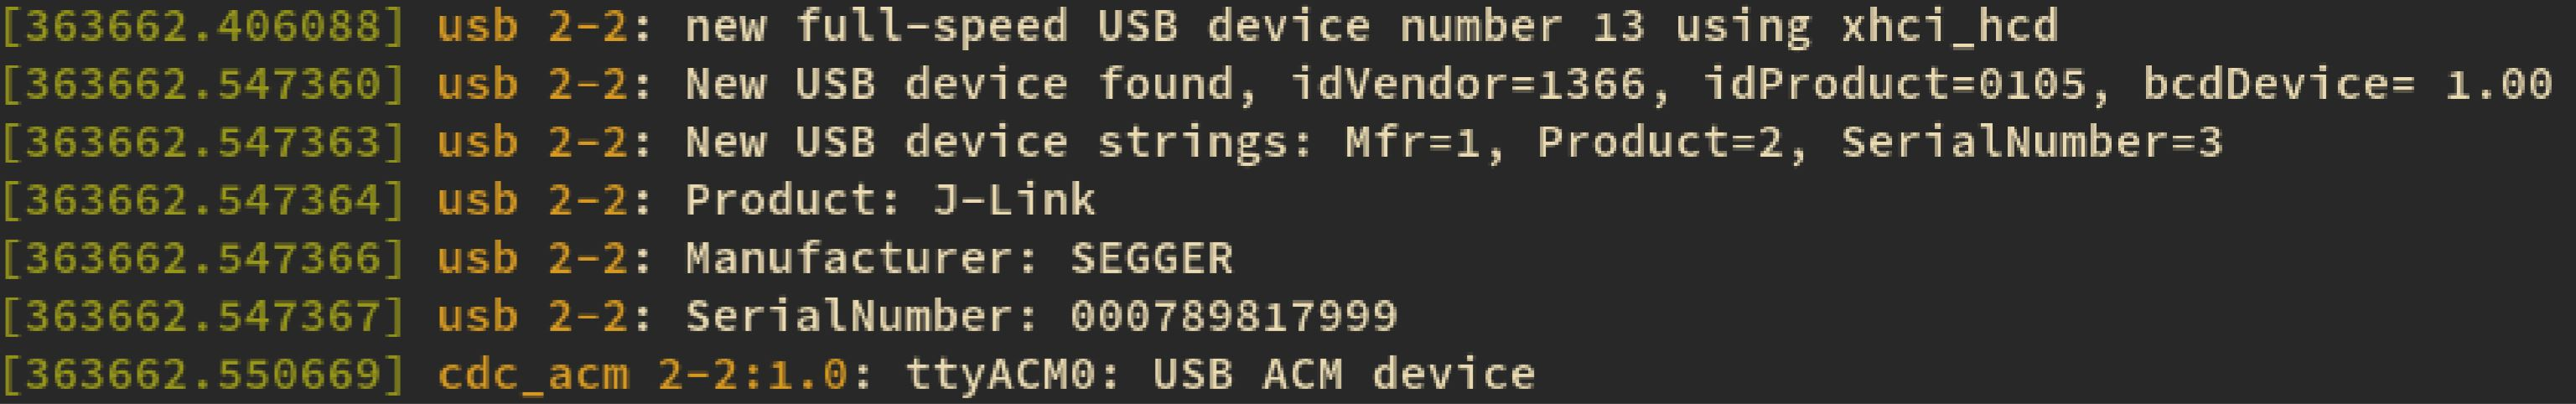
\includegraphics[scale=0.4]{figures/picocom.JPG}
        \caption{Output fra terminalen.}
        \label{fig:picocom-terminal-output}
    \end{figure}
    
    \item Ta nå navnet som utviklingskitet ble tildelt av operativsystemet (i dette eksemplet har utviklingskitet fått navnet "\verb|ttyACMO|") og prøv det etter "\verb|/dev/|" i \verb|picocom|.
    
\end{enumerate}

\section{Appendiks - Debugging av mikrokontrollere}
\label{app:Debugging}

Her vil du få en rask introduksjon om hvordan debugging av mikrokontrollere fungerer, med et spesielt fokus på debugging av Nordic nRF52 DK i et moderne utviklingsmiljø.

\subsection{Serial Wire Debug (SWD)}

Når vi debugger et program som kjører på datamaskinen vår, har vi direkte tilgang til prosessoren vi programmerer. På mikrokontrollere må vi kommunisere gjennom ett eller flere kommunikasjonslag for å hente informasjon fra prosessoren til mikrokontrolleren. Mikrokontrollere (som nRF52832 SoC) har som regel et grensesnitt for å dele informasjon med eksterne enheter. Dersom vi ser på \verb|PCA10040_Schematic_And_PCB|, kan vi legge merke til to pins, SWDIO (26) og SWDCLK (25), som går fra target MCU (nRF52832) og videre til interface MCU (nRF5340). Disse to portene betegner det fysiske grensesnittet for Serial Wire Debug (SWD). Dette er en protokoll som definerer hvordan vi kan programmere prosessoren vår (ARM Cortex-M4), men også hvordan vi kan henter informasjon fra prosessoren. 

\begin{figure}[ht]
    \centering
    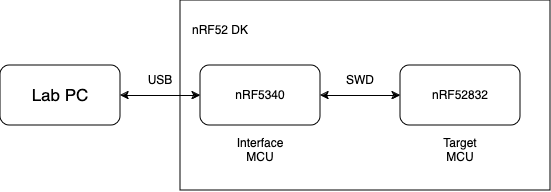
\includegraphics[scale=0.60]{Main/figures/nrf52_debug_swd.png}
    \caption{Visualisering av kommunikasjonslag}
    \label{fig:debugging_swd}
\end{figure}

For å få videresende informasjonen vi får fra mikrokontrolleren må vi bruke et program på interface MCU som fungerer som et kommunikasjonslag mellom vår datamaskin og target MCU. nRF52 DK sin interface MCU (nRF5340) er utstyrt med J-Link, som er et kraftig verktøy for feilsøking og programmering av target MCU (nRF52832). Den innebygde feilsøkingsprogrammet støtter feilsøking i monitormodus, en funksjon som gjør det mulig for utviklere å samhandle med mikrokontrollerens kjøringsmiljø i sanntid. Dette er spesielt nyttig ved feilsøking av komplekse problemer som krever mulighet til å inspisere og endre mikrokontrollerens tilstand (registerverdier etc.) mens koden kjører. Enkelt forklart blir denne informasjonen delt med interface MCU, som kan tolke og videresende informasjonen over til vår maskin over USB (se figur \ref{fig:debugging_swd}). 


\subsection{GDB Server}

For å gjøre nytte av informasjonen vil blir sendt av den innebygde debuggeren (interface MCU) på mikrokontrolleren bruker vi tjenere som kan tolke informasjonen for oss. I vårt tilfelle er dette en GDB-server. Dette gjør slik at andre programmer, som f.eks. VSCode (eller en vanlig GDB session) kan kommunisere med mikrokontrolleren over TCP/IP-forbindelse. `Server'-enheten seg av kommunikasjon med både GDB, og hardware, ved å abstrahere bort hvilken type forbindelse man har mellom datamaskinen og plattformen som blir debugget. I prinsippet kan `Server' være hva som helst, så lenge det er et program som støtter kommandoer fra GDB, og er i stand til å kommunisere med målhardwaret. 


\subsection*{Debugging med VSCode}

Mange foretrekker å debugge og programmere i en moderne IDE som VSCode. Vi har derfor laget et utviklingsmiljø vedlagt i hver oppgave. Utviklingsmiljøet kan også lastes ned ved \verb|git clone| \href{https://github.com/ITK-TTK4235/nrf52dk-environment}{via denne lenken her}. Utviklingsmiljøet baserer seg på utvidelsen \href{https://open-vsx.org/extension/marus25/cortex-debug}{Cortex-Debug}, som bruker J-Link GDB for å kommunisere med mikrokontrolleren over USB. Sørg for at \verb|.vscode|-mappen ligger i samme mappe som \verb|.build_system|. Begge disse mappene er "skjulte", som vil si at du må bruke \verb|ls -a| for å se dem i et terminalvindu. Åpne så oppgavemappen i VSCode (dette kan du gjøre med kommandoen \verb|code .| ). VSCode vil så be deg om å laste ned utvidelsen \verb|Cortex-debug|. Etter å ha installert denne kan du trykke på \verb|Run and Debug|-fanen for å så debugge programmet. For mer informasjon om hvordan man debugger nRF52 DK i VSCode, ta en titt på Github-repositoryet \href{https://github.com/ITK-TTK4235/nrf52dk-environment}{nrf52dk-environment}.

\subsection{Laste opp eksempelkode}
I det utdelte utviklingsmiljøet \verb|nrf52dk-environment| ligger det eksempelkode som dere kan kompilere og flashe ved å kalle \verb|make| og \verb|make flash|. Koden vil blinke LED 1 med jevne intervaller. 


